% ======================================================================
\subsection{\Fv s}

% ----------------------------------------------------------------------
\begin{frame}[shrink]
  \frametitle{Floquet exponents}

  
  {\centering
    \includegraphics[width=0.6\textwidth]{ppo1spectrum64}
    \par}
  {\scriptsize \centering
    Floquet exponents of \PPO{10.25}.
    The dashed line (green) is
    $q_{k}^{2}-q_{k}^{4}$. The inset is a magnification of the region
    containing the 8 leading exponents.
    \par}

  {\centering
    \htgc{The smallest multiplier : $10^{-27\,067}$.}

    $
      \ExpaEig_{j} = \exp(\period{p}\Lyap^{(j)}_p)\
      = \exp(\period{p}\eigRe[j] + i\theta_j)
    $
  \par}

\end{frame}

% ----------------------------------------------------------------------
\begin{frame}[shrink]%[allowframebreaks]
  \frametitle{\Fv s}

  {\centering
    \begin{minipage}{0.3\textwidth}
      \centering \small{\texttt{(a)}}
      \includegraphics[width=\textwidth]{ksppo1fvt0v1r}
    \end{minipage}
    \begin{minipage}{0.3\textwidth}
      \centering \small{\texttt{(b)}}
      \includegraphics[width=\textwidth]{ksppo1fvt0v5}
    \end{minipage} \\
    \begin{minipage}{0.3\textwidth}
      \centering \small{\texttt{(c)}}
      \includegraphics[width=\textwidth]{ksppo1fvt0v10}
    \end{minipage}
    \begin{minipage}{0.3\textwidth}
      \centering \small{\texttt{(d)}}
      \includegraphics[width=\textwidth]{ksppo1fvt0v30}
    \end{minipage}
    \par}
  { \scriptsize \centering 
    \Fv s of \PPO{10.25} at $t=0$. \\
    The real part of  the
    (a) 1st, (b )$5$th, (c) $10$th, and (d) $30$th \Fv s.
  }
\end{frame}

% ----------------------------------------------------------------------
\begin{frame}[shrink]%[allowframebreaks]
  \frametitle{\Fv s  along the orbit}
 
  {\centering
    \begin{minipage}{.115\textwidth}
      \centering \small{\texttt{(a)}}
      \includegraphics[width=\textwidth]{ppo1Fv1_64}
    \end{minipage}
    \begin{minipage}{.115\textwidth}
      \centering \small{\texttt{(b)}}
      \includegraphics[width=\textwidth]{ppo1Fv5_64}
    \end{minipage}
    \begin{minipage}{.115\textwidth}
      \centering \small{\texttt{(c)}}
      \includegraphics[width=\textwidth]{ppo1Fv10_64}
    \end{minipage}
    \begin{minipage}{.115\textwidth}
      \centering \small{\texttt{(d)}}
      \includegraphics[width=\textwidth]{ppo1Fv30_64}
    \end{minipage}
    \begin{minipage}{.115\textwidth}
      \centering \small{\texttt{(e)}}
      \includegraphics[width=\textwidth]{rpo1Fv1_64}
    \end{minipage}
    \begin{minipage}{.115\textwidth}
      \centering \small{\texttt{(f)}}
      \includegraphics[width=\textwidth]{rpo1Fv4_64}
    \end{minipage}
    \begin{minipage}{.115\textwidth}
      \centering \small{\texttt{(g)}}
      \includegraphics[width=\textwidth]{rpo1Fv10_64}
    \end{minipage}
    \begin{minipage}{.115\textwidth}
      \centering \small{\texttt{(h)}}
      \includegraphics[width=\textwidth]{rpo1Fv30_64}
    \end{minipage}
    \par}
  {\scriptsize \centering
    (a) $\sim$ (d) : the 1st (real part), 5th, 10th and 30th \Fv\ along
    \PPO{10.25} for one prime period.
    (e) $\sim$ (h) : the 1st, 4th (real part), 10th (imaginary part) 30th (imaginary part)
    \Fv\ along \RPO{16.31} for one prime period.
  }

\end{frame}

% ----------------------------------------------------------------------
% \begin{frame}[shrink]%[allowframebreaks]
%   \frametitle{Power spectra of \Fv s}
  
%   {\centering
%     \begin{minipage}{.47\textwidth}
%       \centering \small{\texttt{(a)}}
%       \includegraphics[width=\textwidth]{ppo1power64}
%     \end{minipage}
%     \begin{minipage}{.47\textwidth}
%       \centering \small{\texttt{(b)}}
%       \includegraphics[width=\textwidth]{rpo1power64}
%     \end{minipage}
%     \par}
%   {\scriptsize \centering
%     The power spectrum of the first 30 \Fv s for \PPO{10.25}
%     (left) and \RPO{16.31} (right)
%     at $t=0$. Red lines correspond to the leading 8 \Fv s; while
%     the blue lines correspond to the left 22 \Fv s with the $i${th} one
%     localized at index $\lceil \frac{i}{2} \rceil$.
%   }
 

% \end{frame}

% ----------------------------------------------------------------------
\begin{frame}%[allowframebreaks]
  \frametitle{Accuracy of \Fv s}

  \PPO{10.25}
  {\centering
    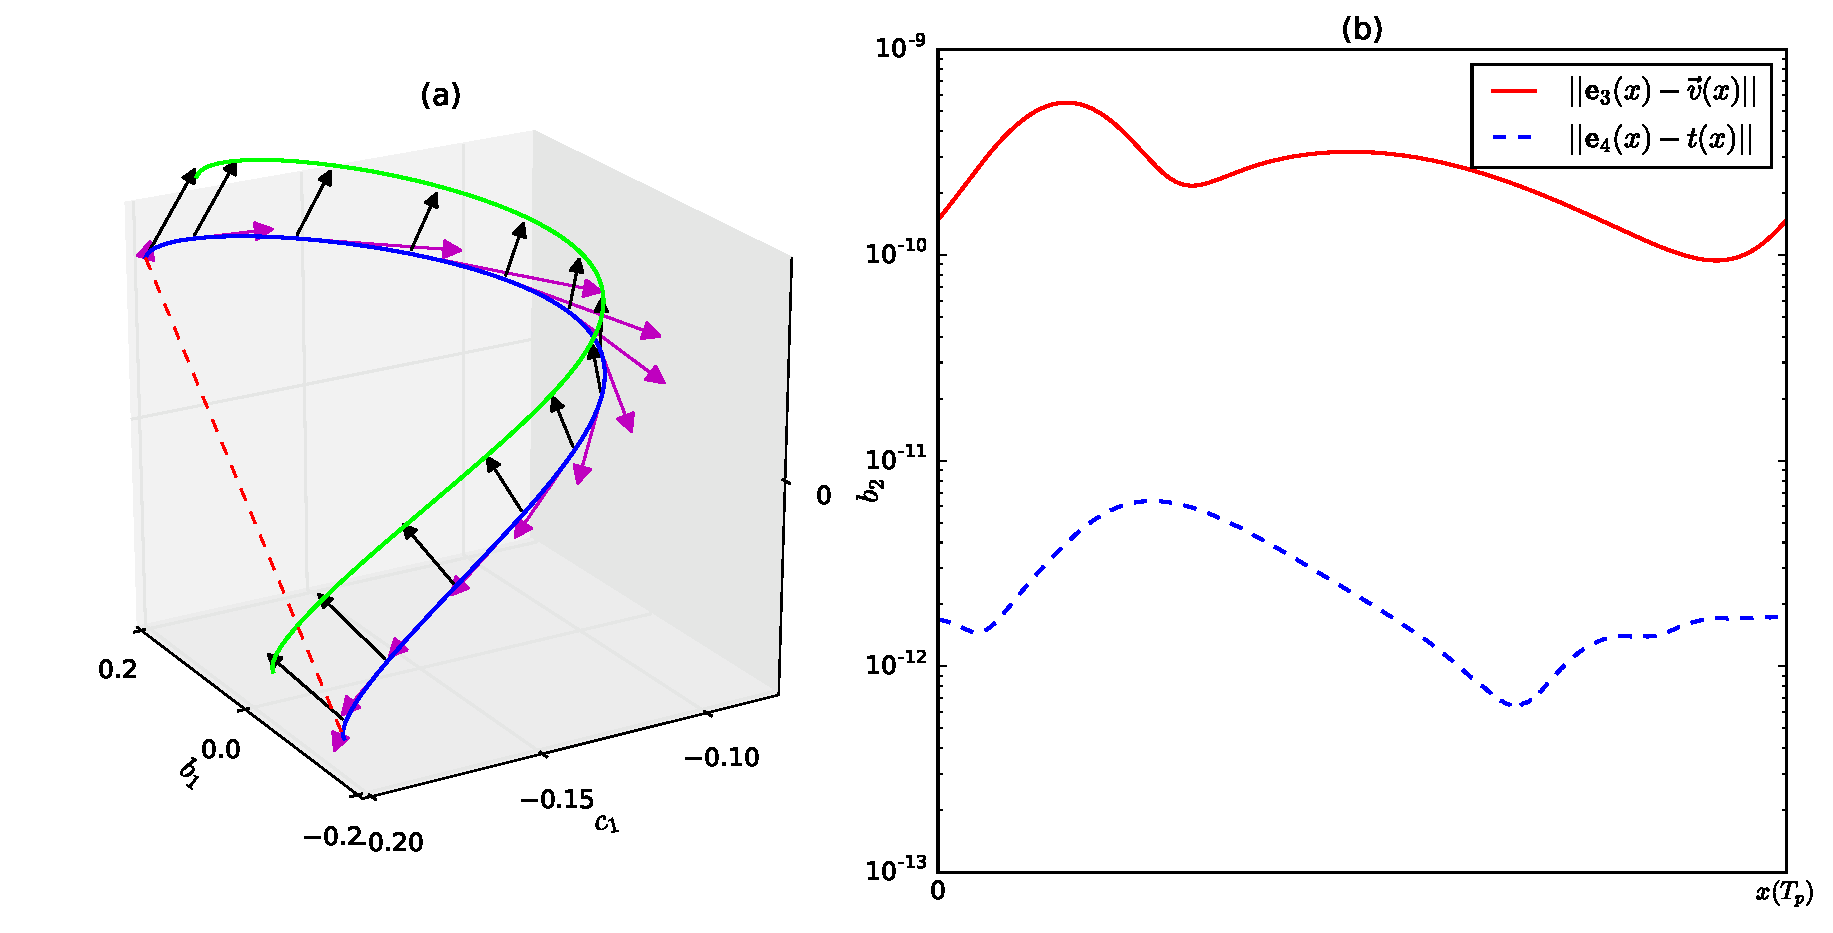
\includegraphics[width=0.8\linewidth]{ppo1vectfield}
    \par}
  {\scriptsize \centering
    Marginal vectors and the associated errors.
    (a) \PPO{10.25} in one period projected onto
    {$[b_1, c_{1}, b_{2}]$}
  }

\end{frame}

% ----------------------------------------------------------------------
\begin{frame}%[allowframebreaks]
  \frametitle{Accuracy of \Fv s}

  \RPO{16.31}
  
  {\centering
    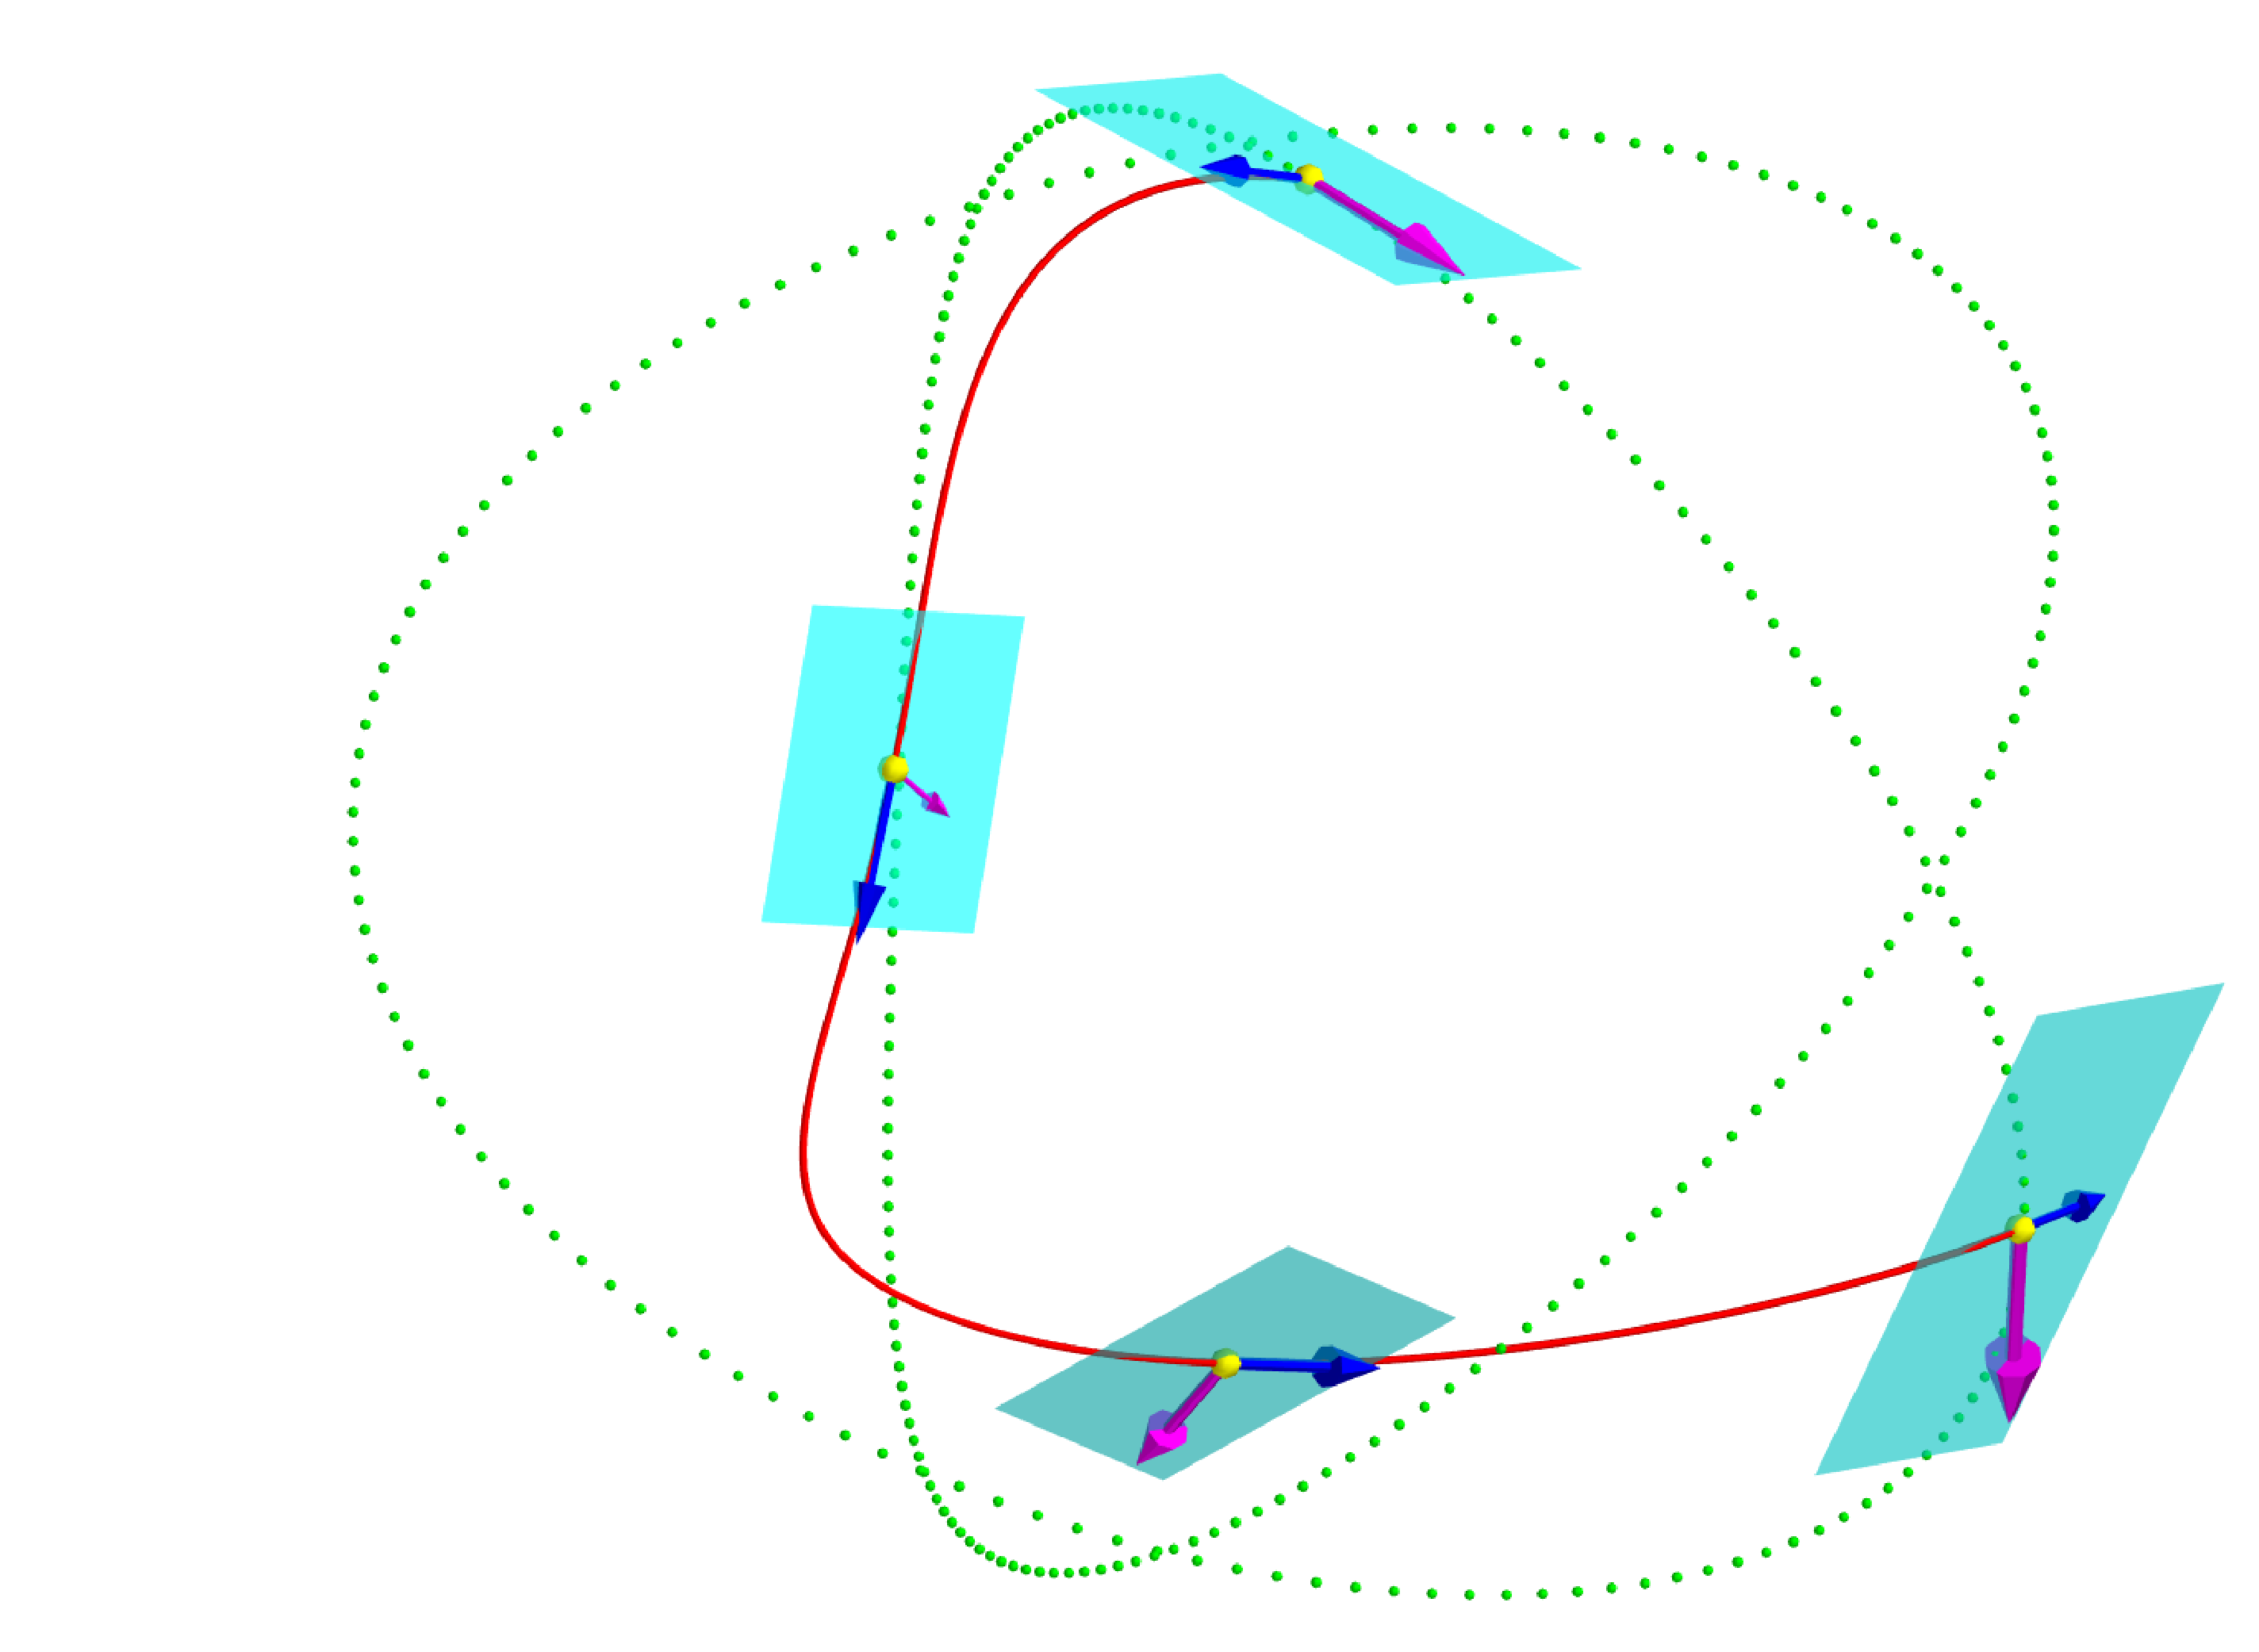
\includegraphics[width=0.7\linewidth]{rpo1_marginal3}
    \par}

\end{frame}

% ----------------------------------------------------------------------
\begin{frame}[shrink]%[allowframebreaks]
  \frametitle{In-slice \JacobianM}

  {\centering
    \includegraphics[width=0.9\linewidth]{jacobian_full_slice}
    \par}
  {\scriptsize \centering 
    Deformations in
    the full {\statesp} and in the \slice.
    \par}
  \[
    \hat{\jMps}\pMatM
    (\sspRed(\zeit_1))\LieEl(\gSpace_1)^{-1}=
    \pMatM(\sspRed(\zeit_2))\LieEl(\gSpace_2)^{-1}\jMps
    \,.
  \]
  \pause
  \htb{
    \[
      \hat{\ExpaEig}_{j} = \ExpaEig_{j} \,, \quad
      \jEigvecRed[j] = \pMatM(\sspRed_p)\LieEl(\gSpace_p)^{-1} \jEigvecRed[j]
      \,.
    \]
  }

\end{frame}
